\documentclass{article}
\usepackage{graphicx}
\usepackage[backend=biber]{biblatex}
\addbibresource{sources.bib}
\usepackage{tikz}
\usepackage{amsmath, amssymb, amsthm}
\usepackage{verbatimbox}
\usepackage{listings}
\usepackage{xcolor}
\usepackage{hyperref}
\usepackage{array}
\usepackage[colorlinks=true, linkcolor=blue, urlcolor=blue, citecolor=blue]{hyperref}

\theoremstyle{definition}
\newtheorem{definition}{Definition}[section]

\theoremstyle{question}
\newtheorem{question}{Key Question}[section]

\title{\vspace{-2.0cm}\textbf{Insights from Discrete Mathematics \\
\LARGE from \emph{Integer Partitions} to \emph{Rooted Trees}}}
\author{\textit{Ethan Li} \\ \small Grade 9, Central Toronto Academy \\ \\ \small Mentored by \normalsize \textit{Claire Zhao}}
\date{May 11, 2024}


\begin{document}

\maketitle

\section{Introduction}

\subsection{Definition of Partitioning}
A partition of a positive integer \(n\) is written as a sum of positive integers. Different orders of the same partitions do not count as separate partitions.

\subsection{Examples}
Let \(P(n)\) output the number of partitions for any number \(n\).\\

\noindent By default, \(P(0)=1\)\\

\noindent 1 can be written as \(1\), hence \(P(1)=1\)\\

\noindent 2 can be written as \(1+1\) and \(2\), hence \(P(2)=2\)\\

\noindent 3 can be written as \(1+1+1\), \(1+2\) and \(3\). \(1+2\) is the same thing as \(2+1\), it is only counted once, making \(P(3) = 3\)\\

\noindent 4 can be written as \(1+1+1+1\), \(1+1+2\), \(1+3\), \(2+2\) and \(4\), which results in \(P(4)=5\)

\subsection{Different Representations of the Partitions}
\subsubsection{Ferrers diagram}

A partition can be represented graphically through a Ferrers diagram, named after British mathematician Norman Macleod Ferrers. For example, \(5=2+2+1\) can be illustrated as follows:\\
\begin{center}
\begin{verbbox}
2 2 1
* * *
* *
\\
\end{verbbox}
\theverbbox
\end{center}

\noindent A conjugate for this diagram can be created by swapping the columns with rows. For example, \(5=3+2\) is represented as:

\begin{center}
\begin{verbbox}
3 2
* *
* *
*
\\
\end{verbbox}
\theverbbox
\end{center}
\noindent Therefore, the conjugate of (2, 2, 1) is (3, 2).
\newline
\newline
If the conjugate of a partition happens to be the same as the partition itself, it is called a self-conjugate. For instance, \(10=(4, 3, 2, 1)\) can be shown as:
\begin{center}
\begin{verbbox}
  4 3 2 1
4 * * * *
3 * * * 
2 * *
1 *
\\
\end{verbbox}
\theverbbox
\end{center}

\subsubsection{Young Diagram}
Alfred Young created the Young Diagram, which is similar to the Ferres diagram but uses squares instead of dots. Although Young diagrams are very similar to Ferres diagrams, they are particularly useful for studying group representation theory and symmetric functions. \\

\noindent \href{https://youtu.be/8qc71j8yhG0}{Animations demo for Young Diagram using Python Manim.}\cite{manim}


\begin{figure}[h]
\centering
\begin{tikzpicture}
    % Partition 4
    \draw (0,0) rectangle (4,1);
    \draw (1,0) -- (1,1);
    \draw (2,0) -- (2,1);
    \draw (3,0) -- (3,1);
    \node at (2, -0.5) {4};

    % Partition 3+1
    \draw (5,0) rectangle (8,1);
    \draw (6,0) -- (6,1);
    \draw (7,0) -- (7,1);
    \draw (5,0) rectangle (6,-1);
    \node at (6.5, -1.5) {3+1};

    % Partition 2+2
    \draw (9,0) rectangle (11,1);
    \draw (9,0) rectangle (11,-1);
    \draw (10,0) -- (10,1);
    \draw (10,-1) -- (10,0);
    \node at (10, -1.5) {2+2};
\end{tikzpicture}
\end{figure}

\begin{figure}[h]
\centering
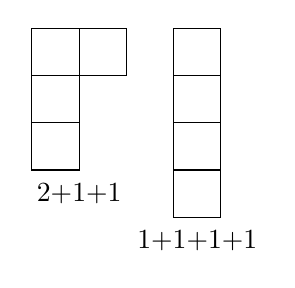
\begin{tikzpicture}[scale=0.6]

    % Partition 2+1+1
    \draw (0,-4) rectangle (2,-3); % Shifted to start at (0, -4)
    \draw (1,-4) -- (1,-3);
    \draw (0,-4) rectangle (1,-5);
    \draw (0,-5) rectangle (1,-6);
    \node at (1, -6.5) {2+1+1};

    % Partition 1+1+1+1
    \draw (3,-4) rectangle (4,-3); % Shifted to start at (3, -4)
    \draw (3,-4) rectangle (4,-5);
    \draw (3,-5) rectangle (4,-6);
    \draw (3,-6) rectangle (4,-7);
    \node at (3.5, -7.5) {1+1+1+1};
\end{tikzpicture}
\caption{Young diagram for all partitions of 4.}
\end{figure}


\newpage
\section{Euler's Generating Function}

\subsection{Intro to Euler's Generating Function}
Euler discovered several theorems related to integer partitioning, but his generating function is particularly notable. It is defined as:

\[
\sum_{n=0}^{\infty} p(n) x^n = \frac{1}{\prod_{p=1}^{\infty} (1-x^p)}, \quad \text{where } |x| < 1
\]

\noindent For instance, to find the number of partitions of 7, we examine the coefficient of \(x^7\).
\[
(1 + x^{1\cdot(1)} + x^{1\cdot(2)} + x^{1\cdot(3)} + \ldots )(1 + x^{2\cdot(1)} + x^{2\cdot(2)} + x^{2\cdot(3)} + \ldots )(1 + x^{3\cdot(1)} + x^{3\cdot(2)} + x^{3\cdot(3)} + \ldots ) \ldots
\]
Expanding above to get \(1 + x + 2x^2 + 3x^3 + 5x^4 + 7x^5 + 11x^6 + 15x^7 + 22x^8 + \ldots\)
\newline
\newline
\noindent Hence, \(P(7)=15\)


\subsection{Euler's Odd-Partitions \& Distinct-Partitions Theorem}
Another interesting theorem by Euler states that the number of odd-partitions is equal to the number of distinct parts:\\

\noindent (1) Odd parts: A partition of any number n which contains only odd numbers.

\noindent (2) Distinct parts: A partition that contains no repeated numbers. \\

\noindent Here is an example to demonstrate this theorem, 5 can be written:
\begin{table}[h]
    \centering 
    \begin{tabular}{|c|c|}
    \hline
    Partition & Type \\
    \hline
    (5) & Odd part, Distinct part \\
    (4, 1) & Distinct part \\
    (3, 2) & Distinct part \\
    (3, 1, 1) & Odd part \\
    (2, 2, 1) & N/A \\
    (2, 1, 1, 1) & N/A \\
    (1, 1, 1, 1, 1) & Odd part \\
    \hline
    \end{tabular}
    \caption{Euler - Types of partitions for Integer 5}
\end{table}
    
\noindent Hence, we have 3 of each and the number of odd parts is equal to the number of distinct parts.

\newpage
\section{Hardy-Ramanujan’s Asymptotic Expression}
In 1918, Godfrey Hardy and Srinivasa Ramanujan developed an asymptotic formula for the number of partitions of a number \( n\), using the circle method along with modular functions to create an asymptotic solution:
\[
p(n) \approx \frac{1}{4n\sqrt{3}} e^{\pi \sqrt{\frac{2n}{3}}} \quad \text{as} \quad n \to \infty
\]
This formula shows the rapid increase in the number of partitions as \( n \) becomes larger.\\

\noindent For example, when plugging in the numbers 20, 50 and 100, we have the following outcomes:\\

\noindent \href{https://youtu.be/UYjqhT5xnsY}{Animations demo for Hardy-Ramanujan’s Asymptotic Expression using Python Manim.}\cite{manim}

\begin{table}[h!] 
    \centering % Centers the table
    \begin{tabular}{|c|c|c|c|}
        \hline
        $n$ & $p(n)$ & $p(n)$ using formula & $p(n)$ using formula$/p(n)$ \\
        \hline
        20 & 627 & 692.3846405 & 1.104281723 \\
        50 & 204226 & 217590.4992 & 1.065439754 \\
        100 & 190569292 & 199280893.3 & 1.045713563 \\
        $\vdots$ & $\vdots$ & $\vdots$ & $\vdots$ \\
        $\infty$ & $\infty$ & $\infty$ & 1 \\
        \hline
    \end{tabular}
    \caption{The outcomes of the Hardy-Ramanujan’s Asymptotic Expression} 
\end{table}


\newpage
\section{The Coins Change Problem}
    \noindent \href{https://youtu.be/PmR1eRswj3A}{Animations demo for Coin Change Combination Problem using Python Manim.}\cite{manim}

    \subsection{The Coins Change Problem}
    \begin{center}
        Question:
        “\textit{In how many ways can you change one dollar?}” \cite{gpolya1956}
    \end{center}
    
    \begin{figure}[h!]
        \centering
        \includegraphics[width=8cm]{images/coins-change.jpg}
        \caption{How many ways can you change one dollar?}
    \end{figure}
    
    \newpage
    \noindent Interpret the coins change problem in mathematical form as follows: \\
    
    \noindent 
    \begin{center}\textbf{\noindent Let \( P_n \) denote the number of ways of paying \( n \) cents \\ with cents, nickels, dimes, quarters, and half dollars.\\ Given \(P_4=1\), \(P_6=2\), and \(P_{10}=4\), what is \(P_{100}\) ?}
    \end{center}
    
    \noindent Now let's explore the various possibilities here. For instance, we could use denominations of 1 cent, 2 cents, 5 cents, and so on, as demonstrated in the diagram below: \\
    
    \noindent In the first diagram, if we interpret each line as the sum of pictures in it, and then consider the product of these five infinite sums, we get the second diagram. Once this is expanded, it gives us the number of different ways of making payments. \\
    
    \noindent For instance, if we take the term with \(2\) coins in line two, it represents paying two nickels. \\
    
    \noindent In order to make this work, we substitute each pictorial variable as a power of a new variable x. The exponent of x would be the joint value of the coins represented by the  picture. Then we get:
    
    \[
    P_0 + P_1 x + P_2 x^2 + \dots + P_n x^n + \dots
    \]
    
    \noindent In above series, the coefficient of \(x^n\) counts the number of different ways of paying the amounts of n cents. This is called the enumerating series. We can substitute the second figure into a \textbf{geometric series} as follows:
    
    \[
    1 + x + x^2 + x^3 + \dots = \frac{1}{1-x}
    \]
    
    \noindent This changes each of the first five lines into a geometric series and equation in the second figure. So we have:
    
    \[
    (1 - x)^{-1}(1 - x^5)^{-1}(1 - x^{10})^{-1}(1 - x^{25})^{-1}(1 - x^{50})^{-1} = P_0 + P_1 x + P_2 x^2 + \dots + P_n x^n
    \]
    
    \noindent This sum is usually termed as the generating function. This function expanded in powers of \(x\) generates the numbers \(P_0, P_1, \dots, P_n\), our starting point. \\
    
    \noindent To get our generating function, we put every single power of \(x\) instead of just the coin values. This gives us all the partitions of an integer. \\
    
    \noindent Now, we have reduced this combinatorial problem to a different kind of problem! We must expand it in powers of \(x\). Let's assume we have already obtained the expansion of the product of the first two factors:
    \[
    (1 - x)^{-1}(1 - x^5)^{-1} = a_0 + a_1 x + a_2 x^2 + \dots
    \] \\
    
    \noindent  We can use this to find the expansion for 3 factors
    \[
    (1 - x)^{-1}(1 - x^5)^{-1}(1 - x^{10})^{-1} = b_0 + b_1 x + b_2 x^2 + \dots
    \]
    This means:
    \[
    a_0 + a_1 x + a_2 x^2 + \dots = (b_0 + b_1 x + b_2 x^2 + \dots)(1 - x^{10})
    \]
    If we compare the coefficients of $x^n$, we find that
    \[
    b_n = a_n + b_{n-10}
    \]
    With this, we can conveniently compute the coefficients of $b_n$ if the coefficients of $a_n$ are already known. \\
    
    \noindent Let's add a table that computes $P_{50}$. The table below represents the coefficients for the series expansions of $(1-x)^{-1}$, $(1-x^5)^{-1}$, $(1-x^{10})^{-1}$, $(1-x^{25})^{-1}$, and $(1-x^{50})^{-1}$: 
    
    \[
    \begin{array}{|c|*{11}{c|}}
    \hline
    n = & 0 & 5 & 10 & 15 & 20 & 25 & 30 & 35 & 40 & 45 & 50 \\
    \hline
    (1 - x)^{-1} & 1 & 1 & 1 & 1 & 1 & 1 & 1 & 1 & 1 & 1 & 1 \\
    \hline
    (1 - x^5)^{-1} & 1 & 2 & 3 & 4 & 5 & 6 & 7 & 8 & 9 & 10 & 11 \\
    \hline
    (1 - x^{10})^{-1} & 1 & 2 & 4 & 6 & 9 & 12 & 16 & 20 & 25 & 30 & 36 \\
    \hline
    (1 - x^{25})^{-1} & 1 & 2 & 4 & 6 & 9 & 13 &  &  &  &  & 49 \\
    \hline
    (1 - x^{50})^{-1} & 1 &  &  &  &  &  &  &  &  &  & 50 \\
    \hline
    \end{array}
    \]
    
    \noindent  This table above yields $P_{50} = 50$, which means one can pay 50 cents in 50 different ways. Although this table only computes up to $P_{50}$, we can continue this computation and verify that $P_{100} = 292$.



\newpage
% Cayley's generating function
    \section{Rooted Trees}
    \subsection{Introduction}
    \begin{definition}
                    A \emph{tree} is a graph consisting of vertices and edges 
            but contains no closed path. A \emph{rooted tree} is a tree with one distinguished vertex called the \emph{root}. A non-root vertex is called a \emph{knot}.
    \end{definition}

\begin{question}
    How many rooted trees with $n$ knots?
\end{question}
        \begin{figure}[h]
            \centering
            \includegraphics[scale=0.5]{images/rooted-tree.png}
            \caption{A rooted tree}
            \label{fig:enter-label}
        \end{figure}

    \subsection{From Trees to Cayley’s Generating Function}
        \begin{figure}[h]
            \centering
            \includegraphics[scale=0.3]{images/rooted-tree.png}
            \label{fig:rooted-tree}
        \end{figure}
        \noindent Let there be $T_n$ such trees, we look for a generating function with 
        $T_n$ as coefficient.
        \begin{equation*} % Changed from equation to align
             T_1x + T_2 x^2 + T_3 x^3 +\cdots = x(1-x)^{-T_1}(1-x^2)^{-T_2}(1-x^3)^{-T_3}\cdots
        \end{equation*}

    \subsection{A Visual Proof}
        \begin{figure}[h]
            \centering
            \includegraphics[scale=0.6]{images/tree1.png}
            \label{fig:enter-label}
        \end{figure}
    Combinatorial insight: a rooted tree consists of \underline{the root} +  
    \begin{enumerate}
        \item some number of $1$-trees
        \item some number of $2$-trees ...
    \end{enumerate}
    where the total number of knots add up to $n$.

\subsection{Important Observation}
        \begin{figure}[h]
            \centering
            \includegraphics{images/tree2.png}
            \caption{A $3$-tree can be chosen $T_3$ different ways!}
            \label{fig:enter-label}
        \end{figure}

    \subsection{Making choices by multiplication}
        \begin{figure}[h]
            \centering
            \includegraphics[scale=0.5]{images/tree3.png}
            \caption{Infinitely many rows: $T_k$ rows for $k$-trees}
            \label{fig:enter-label}
        \end{figure}
        Insight: when you expand this product you are actually making choices

\newpage

    \subsection{Visual generating function}
        \begin{figure}[h]
            \centering
            \includegraphics[scale=0.6]{images/tree5.png}
            \caption{convert pictures into algebra}
            \label{fig:enter-label}
        \end{figure}

    \begin{align*}
        & T_1x + T_2 x^2 + T_3 x^3 +\cdots \\
        =\,  & \underbrace{x}_{\text{this $x$ accounts for the root}}(1-x)^{-T_1}(1-x^2)^{-T_2}(1-x^3)^{-T_3}\cdots
    \end{align*}


    \newpage
    \section{Sources Cited}
    % \printbibliography[heading=bibintoc]
    \printbibliography

\end{document}
